\documentclass[10pt,a4paper]{article}
\usepackage[utf8]{inputenc}
\usepackage{amsmath}
\usepackage{amsfonts}
\usepackage{amssymb}
\usepackage{graphicx}
\usepackage{hyperref}
\usepackage{caption}
\usepackage{subcaption}

\usepackage{listings}
\usepackage{color}

\definecolor{dkgreen}{rgb}{0,0.6,0}
\definecolor{gray}{rgb}{0.5,0.5,0.5}
\definecolor{mauve}{rgb}{0.58,0,0.82}

\lstset{frame=tb,
  language=Python,
  aboveskip=3mm,
  belowskip=3mm,
  showstringspaces=false,
  columns=flexible,
  basicstyle={\small\ttfamily},
  numbers=none,
  numberstyle=\tiny\color{gray},
  keywordstyle=\color{blue},
  commentstyle=\color{dkgreen},
  stringstyle=\color{mauve},
  breaklines=true,
  breakatwhitespace=true,
  tabsize=3
}


\begin{document}

%Proposal follows a well-organized structure and would be readily understood by its intended audience. Each section is written in a clear, concise and specific manner. Few grammatical and spelling mistakes are present. All resources used and referenced are properly cited.

\begin{titlepage}
	\centering
	\vspace{1cm}
	{\scshape\Large ED3S: Machine Learning Project \par}
	\vspace{1.5cm}
	{\huge\bfseries Image classification with PASCAL VOC dataset \par}
	\vspace{1.5cm}
	{\Large Author: Oscar Javier Hernandez\par}
	\vfill

% Bottom of the page
	{\large \today\par}
\end{titlepage}

\section{Definition}
%(approx. 1-2 pages)
\subsection{Project Overview}\label{sec: overview}
%In this section, look to provide a high-level overview of the project in layman’s terms. Questions to ask yourself when writing this section:
%
%Has an overview of the project been provided, such as the problem domain, project origin, and related datasets or input data?
%Has enough background information been given so that an uninformed reader would understand the problem domain and following problem statement?

\begin{itemize}
\item {\bf What problem is solved by your intended predictive model?}\\ 
The problem that I have chosen to tackle is the object classification task using the Pascal VOC dataset. For the sake of time I focus on building classifier with four object categories; person, dog, cat, and car. I will outline the architectures of the implemented deep neural networks that I trained for this purpose, the data preprocessing steps that I took and discuss the results.

\item {\bf Why is it important to solve your particular problem?} \\
This particular problem is important to solve because it has numerous real-world applications. For example, self-driving cars use sophisticated algorithms and equipment to map out their environment and in order to take appropriate actions on the road, these cars need algorithms that can classify objects on-the-fly. If the classifier detects animals on the road, it will behave differently depending on the type of animal identified. Small animals, like cats and dogs may have a tendency to run into the road unexpectedly and so the car will drive more carefully than when the animals it identified are humans which are less prone to running onto the road. Of course the usefulness of this type of classifier is not limited to self-driving cars and can be used in other applications, which make this problem useful and important to solve.

\item {\bf How is the data representative of the learning problem?}\\
The PASCAL VOC dataset contains 9963 images, with 20 object classes in total. To simplify the problem, the four categories that I have chosen are are the subsets \lstinline{person,cat,dog,car}. The data is representative of the learning problem since we have images containing objects that are separated into their specific category so that the machine learning model can be taught to recognize those categories. 

\item {\bf How would the estimations of the model be used?}\\
The goal for this image classifier, in the case of the self-driving car example, would be for the self-driving vehicle to supply images via its cameras to the classifier, which will then return the object category to the vehicles computer on the fly. The algorithms in the vehicles computer system would then take the appropriate actions based on the results. However, in general the machine learning model would act as a black box, which is fed images and then outputs the class labels, therefore, this algorithm can also be used as a web app where users upload the image and the application returns the category.
\end{itemize}
 

\newpage
\section{Analysis}
%(approx. 2-4 pages)

\subsection{Data Preprocessing}
%In this section, you will be expected to analyze the data you are using for the problem. This data can either be in the form of a dataset (or datasets), input data (or input files), or even an environment. The type of data should be thoroughly described and, if possible, have basic statistics and information presented (such as discussion of input features or defining characteristics about the input or environment). Any abnormalities or interesting qualities about the data that may need to be addressed have been identified (such as features that need to be transformed or the possibility of outliers). Questions to ask yourself when writing this section:
%
%If a dataset is present for this problem, have you thoroughly discussed certain features about the dataset? Has a data sample been provided to the reader?
%If a dataset is present for this problem, are statistics about the dataset calculated and reported? Have any relevant results from this calculation been discussed?
%If a dataset is not present for this problem, has discussion been made about the input space or input data for your problem?
%Are there any abnormalities or characteristics about the input space or dataset that need to be addressed? (categorical variables, missing values, outliers, etc.)

I used pandas to load the files:\\ 
\lstinline{person_test.txt,cat_test.txt,dog_test.txt,car_test.txt}\\
into a data frame where each row contains the \lstinline{image\_ID} followed by values indicating whether the image contains a person, dog, cat or car (True = 1, False = -1). In addition we process the data and ensure that all of the objects in the dataframe are mutually exclusive. Therefore each image will belong to only one category. I performed this step to attempt to make the training process easier for the classifier, since it would be trained to produce results for only one unique class label  for each image during the training process. The first few entries of this dataframe are given below,
\begin{lstlisting}
   img_ID  is_person  is_dog  is_cat  is_car
0  002846          1      -1      -1      -1
1  002582          1      -1      -1      -1
2  004306         -1       1      -1      -1
3  001748          1      -1      -1      -1
4  005074         -1      -1      -1       1
...
\end{lstlisting}
After filtering the data to make the image categories mutually exclusive, the number of objects in each class are
\begin{lstlisting}
The total number of images:  2660
Number of Persons:  1619
Number of Dogs:  298
Number of Cats:  278
Number of Cars:  465
\end{lstlisting}
I noticed that the category \lstinline{person} has significantly more objects than the other classes. During training, this may introduce a bias in our classifier and as a result of the large number of members in that category it may be better at detecting people than other objects. Therefore, to correct this problem, I chose to remove random images from the \lstinline{person} category until only 500 are left. Once this is complete, my code splits the remaining data set into 80$\%$ training and 20$\%$ validation sets. A bash script will then be generated by the Jupyter notebook that creates the \lstinline{testing, validation} folders which contain subfolders for each object category. The bash script will also place the appropriate copies of images into appropriate subfolders. Below I show an example of the new data frame, with the more balanced sets,
\begin{lstlisting}
=========================================
dropped:  1119
new person number:  500
new dog number:  298
new cat number:  278
new car number:  465
New Dataframe 1541
   img_ID  is_person  is_dog  is_cat  is_car
0  007342          1      -1      -1      -1
1  007001         -1      -1      -1       1
2  002821          1      -1      -1      -1
3  004874          1      -1      -1      -1
4  006394         -1      -1       1      -1
=========================================
\end{lstlisting}
After improving the balance and splitting the data into training/validation the total number of images that went these categories are 
\begin{lstlisting}
Training set size:  1233
Validation set size:  308
\end{lstlisting}
Because the image sets are still fairly small I used image augmentation to generate more training samples from the data set. This was accomplished with the augmentation features in Keras in the following code snippet.

\begin{lstlisting}
train_datagen = ImageDataGenerator(
    rotation_range=50.,
    width_shift_range = 0.2,
    height_shift_range = 0.2,
    rescale=1. / scale,
    shear_range=0.2,
    zoom_range=0.2,
    horizontal_flip=True,
    vertical_flip = True
)


train_generator = train_datagen.flow_from_directory(
    train_data_dir,
    target_size=(img_width, img_height),
    batch_size=batch_size,
    class_mode='categorical')
\end{lstlisting}

One important parameter in the above code snippet is the \lstinline{scale} parameter. This parameter will rescale all images to a particular size. This parameter was treated as a hyperparameter for the models and the values of the parameter that I chose to try were 128 and 256. Larger parameters were run, but due to limitations in computing resources, I was not able to retrieve those results. As shown in the Results section this parameter had an impact on the final models.

\newpage
\subsection{Algorithms and Techniques}
%In this section, you will need to discuss the algorithms and techniques you intend to use for solving the problem. You should justify the use of each one based on the characteristics of the problem and the problem domain. Questions to ask yourself when writing this section:
%
%Are the algorithms you will use, including any default variables/parameters in the project clearly defined?
%Are the techniques to be used thoroughly discussed and justified?
%Is it made clear how the input data or datasets will be handled by the algorithms and techniques chosen?

\begin{itemize}
\item {\bf What classes of learning algorithms you have used, and why?}\\
Because this is an image classification problem, I chose to use convolutional neural network architectures.
Convolutional NNs have been shown to outperform traditional machine learning methods for image classification Ref.~\cite{Krizhevsky_2012} and represent the most current state-of-the-art methods for this problem as described in Ref.~\cite{Russakovsky_2015}. For this reason I have chosen to use CNNs for my project.
\end{itemize}

All models were implemented using Keras. For the architecture of the neural network I chose to try three different methods. The first is a simple benchmark model, consisting of a convolutional network followed by a max pooling layer and then a dense layer with a softmax output. More complicated models should outperform this very simple model. The summary of this network is given below (model 0) and illustrated in Fig.~\ref{fig: model0},\\
\begin{lstlisting}
Model 0
_________________________________________________________________
Layer (type)                 Output Shape              Param #   
=================================================================
conv2d_24 (Conv2D)           (None, 254, 254, 32)      896       
_________________________________________________________________
activation_20 (Activation)   (None, 254, 254, 32)      0         
_________________________________________________________________
max_pooling2d_18 (MaxPooling (None, 127, 127, 32)      0         
_________________________________________________________________
flatten_10 (Flatten)         (None, 516128)            0         
_________________________________________________________________
dense_13 (Dense)             (None, 4)                 2064516   
_________________________________________________________________
activation_21 (Activation)   (None, 4)                 0         
=================================================================
Total params: 2,065,412
Trainable params: 2,065,412
Non-trainable params: 0
_________________________________________________________________
\end{lstlisting}

For the next model, denoted as model 1, I tried the architecture that was suggested in the Keras blog article \cite{Chollet_2016}. This architecture consists of sequences of convolutional layers followed by an activation layer and max pooling. This pattern is repeated three times, before the output is flattened and fed through two dense layers which end in a softmax activation output. The model is regulated with dropout layers. The schematic of this network is shown below, and illustrated in Fig.~\ref{fig: model1}.


\newpage
\begin{lstlisting}
Model 1
_________________________________________________________________
Layer (type)                 Output Shape              Param #   
=================================================================
conv2d_25 (Conv2D)           (None, 254, 254, 32)      896       
_________________________________________________________________
activation_22 (Activation)   (None, 254, 254, 32)      0         
_________________________________________________________________
max_pooling2d_19 (MaxPooling (None, 127, 127, 32)      0         
_________________________________________________________________
conv2d_26 (Conv2D)           (None, 125, 125, 32)      9248      
_________________________________________________________________
activation_23 (Activation)   (None, 125, 125, 32)      0         
_________________________________________________________________
max_pooling2d_20 (MaxPooling (None, 62, 62, 32)        0         
_________________________________________________________________
conv2d_27 (Conv2D)           (None, 60, 60, 64)        18496     
_________________________________________________________________
activation_24 (Activation)   (None, 60, 60, 64)        0         
_________________________________________________________________
max_pooling2d_21 (MaxPooling (None, 30, 30, 64)        0         
_________________________________________________________________
flatten_11 (Flatten)         (None, 57600)             0         
_________________________________________________________________
dense_14 (Dense)             (None, 64)                3686464   
_________________________________________________________________
activation_25 (Activation)   (None, 64)                0         
_________________________________________________________________
dropout_11 (Dropout)         (None, 64)                0         
_________________________________________________________________
dense_15 (Dense)             (None, 4)                 260       
_________________________________________________________________
activation_26 (Activation)   (None, 4)                 0         
=================================================================
Total params: 3,715,364
Trainable params: 3,715,364
Non-trainable params: 0
_________________________________________________________________
\end{lstlisting}

\newpage
\noindent
The last model that I tried was the the VGG-like convnet suggested in \cite{KerasDocs}. This model consists of sequences of two consecutive convolutional layers followed by a max pooling layer. There are three such sequences, which at the end are flattened and fed into a dense layer followed by a softmax output layer. This model, denoted as model 2, is summarized below and illustrated in Fig.~\ref{fig: model2}.
\begin{lstlisting}
Model 2
________________________________________________________________
Layer (type)                 Output Shape              Param #   
=================================================================
conv2d_46 (Conv2D)           (None, 256, 256, 32)      896       
_________________________________________________________________
conv2d_47 (Conv2D)           (None, 254, 254, 32)      9248      
_________________________________________________________________
max_pooling2d_31 (MaxPooling (None, 127, 127, 32)      0         
_________________________________________________________________
dropout_24 (Dropout)         (None, 127, 127, 32)      0         
_________________________________________________________________
conv2d_48 (Conv2D)           (None, 127, 127, 64)      18496     
_________________________________________________________________
conv2d_49 (Conv2D)           (None, 125, 125, 64)      36928     
_________________________________________________________________
max_pooling2d_32 (MaxPooling (None, 62, 62, 64)        0         
_________________________________________________________________
dropout_25 (Dropout)         (None, 62, 62, 64)        0         
_________________________________________________________________
conv2d_50 (Conv2D)           (None, 62, 62, 64)        36928     
_________________________________________________________________
conv2d_51 (Conv2D)           (None, 60, 60, 64)        36928     
_________________________________________________________________
max_pooling2d_33 (MaxPooling (None, 30, 30, 64)        0         
_________________________________________________________________
dropout_26 (Dropout)         (None, 30, 30, 64)        0         
_________________________________________________________________
flatten_15 (Flatten)         (None, 57600)             0         
_________________________________________________________________
dense_22 (Dense)             (None, 512)               29491712  
_________________________________________________________________
dropout_27 (Dropout)         (None, 512)               0         
_________________________________________________________________
dense_23 (Dense)             (None, 4)                 2052      
=================================================================
Total params: 29,633,188
Trainable params: 29,633,188
Non-trainable params: 0
_________________________________________________________________
\end{lstlisting}

\newpage
\section{Results}
In Figs \ref{fig: Final results 128} and \ref{fig: Final results 256} the results of training the three models for 80 epochs are plotted for image scale sizes of 128 and 256, respectively. 

\begin{figure}[h]
\centering
\begin{subfigure}{.7\textwidth}
  \centering
  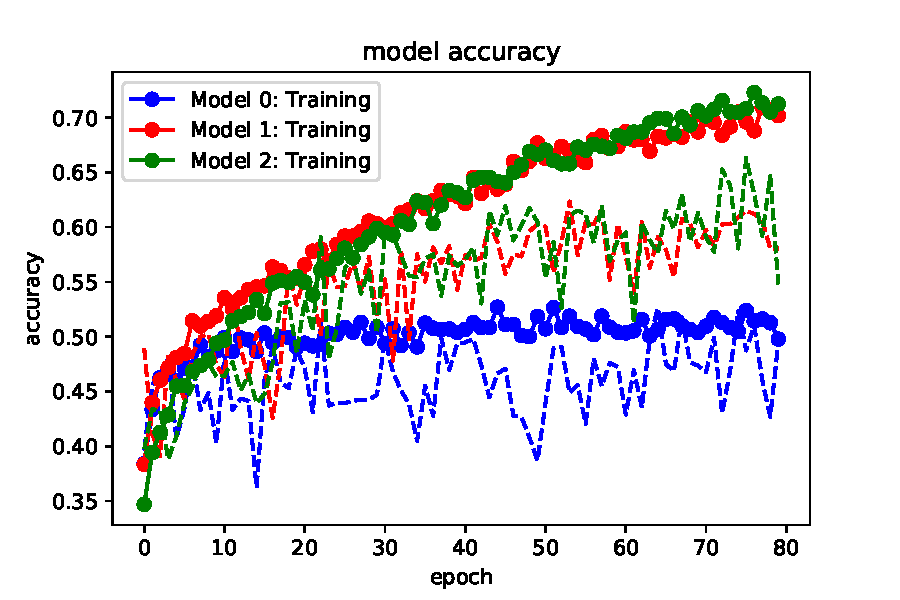
\includegraphics[scale=0.5]{accuracy_vs_epoch_128.pdf}
  \caption{The accuracy of the model vs epoch for\\ three models.}
  \label{fig:sub1 128}
\end{subfigure}%
\begin{subfigure}{.6\textwidth}
  \centering
  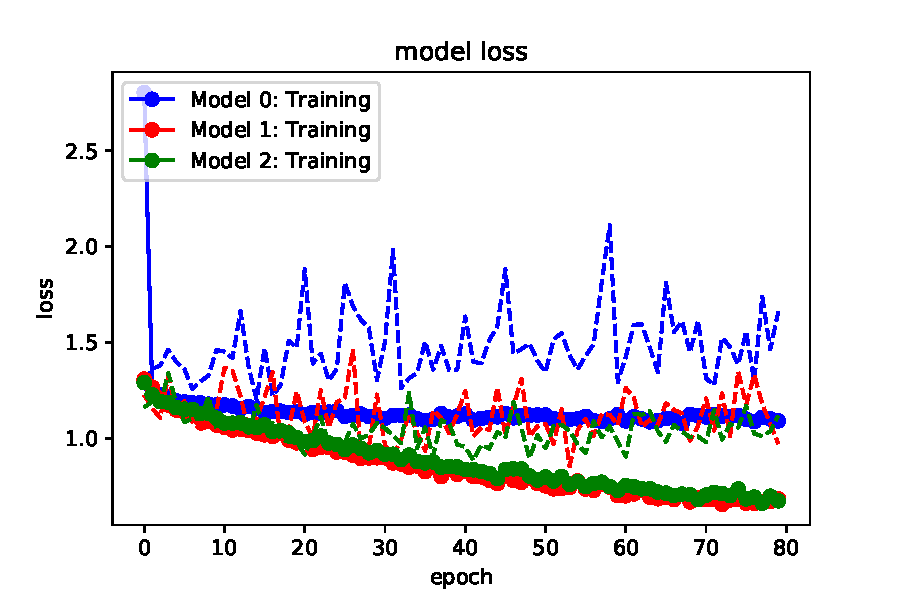
\includegraphics[scale=0.5]{loss_vs_epoch_128.pdf}
  \caption{The loss of the model vs epoch for\\ the three models.}
  \label{fig:sub2 128}
\end{subfigure}
\caption{The results for the three models using \lstinline{scale=128} factor. The solid lines represent the value of the metrics on the training set, while the dashed lines represent the scores on the validation set.}
\label{fig: Final results 128}
\end{figure}

\begin{figure}[h]
\centering
\begin{subfigure}{.7\textwidth}
  \centering
  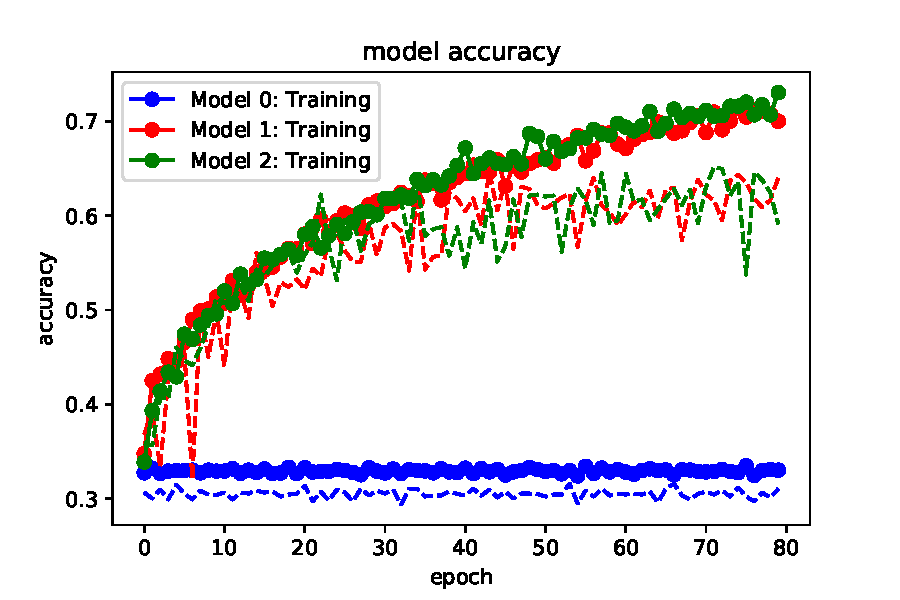
\includegraphics[scale=0.5]{accuracy_vs_epoch_256.pdf}
  \caption{The accuracy of the model vs epoch for\\ three models.}
  \label{fig:sub1 256}
\end{subfigure}%
\begin{subfigure}{.6\textwidth}
  \centering
  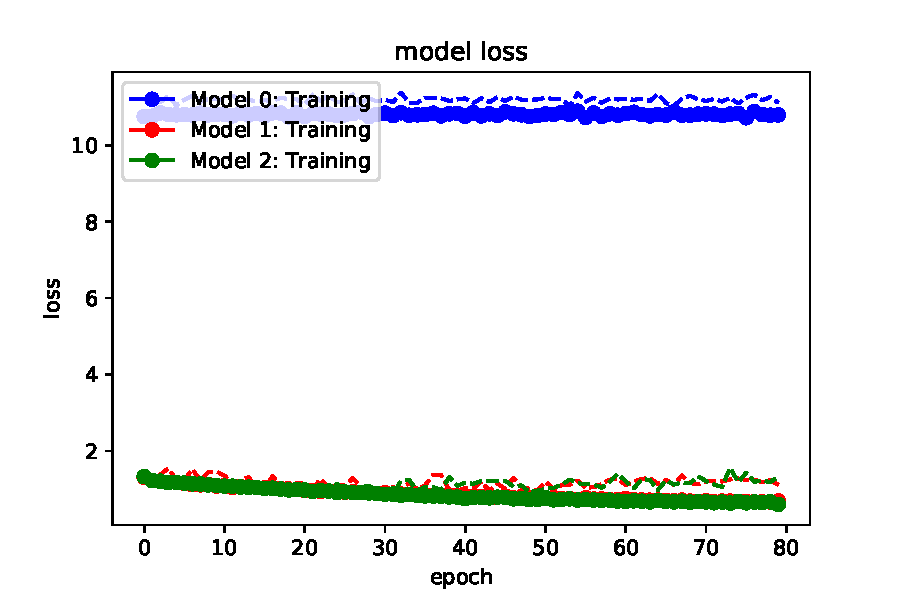
\includegraphics[scale=0.5]{loss_vs_epoch_256.pdf}
  \caption{The loss of the model vs epoch for\\ the three models.}
  \label{fig:sub2 256}
\end{subfigure}
\caption{The results for the three models using \lstinline{scale=256} factor. The solid lines represent the value of the metrics on the training set, while the dashed lines represent the scores on the validation set.}
\label{fig: Final results 256}
\end{figure}

\begin{table}[h]
\centering
\begin{tabular}{c|cc|cc|c}
Model & Training accuracy &  Validation accuracy & Training loss  & Validation loss & Image scale \\ \hline
0 & 0.52  & 0.52 & 1.10 & 1.54 & 128    \\
0 & 0.33  & 0.30 & 10.8 & 11.2 & 256    \\ \hline
1 & 0.71  & 0.69 & 0.67 & 1.14 & 128    \\
1 & 0.71  & 0.62 & 0.67 & 1.20 & 256   \\ \hline
2 & 0.70  & 0.64 & 0.68 & 1.05 & 128    \\
2 & 0.72  & 0.62 & 0.65 & 1.23 & 256 \\ \hline
\end{tabular}
\caption{The accuracy and losses for the training and validation sets for the three different CNN models.}
\label{Table: table1}
\end{table}
In Table \ref{Table: table1} the results of the three models are summarized using image scale parameters of 128 and 256, respectively. These metrics were produced by taking the average of the last four epoch values. The baseline model 0, was the worst performing algorithm as expected. In addition, this model performed better when using a smaller image scale. Model 1 and model 2 both outperformed the baseline model by about 20$\%$ and $50\%$ for image scale parameters 128 and 256, respectively. Both of these models achieved a training set accuracy of about $70\%$ on the training sets and above $60\%$ on the validation sets. Figs \ref{fig:sub1 128} and \ref{fig:sub1 256} show that the accuracies on the validation sets (dotted lines) have plateaued and that more training epochs will not improve the performance, with the exception of model 1, scale=128 shown in red in Fig.~\ref{fig:sub1 128}. However it appears that for all models and scales, the accuracies on the training set are still increasing. The different convergence behaviors between testing and validation sets seem to indicate that, with the exception of model 1 , scale=128, the models are overfitting. This could be overcome by using more aggressive dropout parameters and adding more data to the training images. We also observe in Figs.~\ref{fig:sub2 128} and \ref{fig:sub2 256} that the losses of all models decreases as the epochs increase, but the losses are much smaller for model 1 and 2, and much higher in general for the baseline model.

The result of this analysis suggests that model 1 with a scale=128 was the best performing model, as the accuracy between training and validation sets were very comparable after 80 epochs. 


\subsection{Conclusion}
In this project, we constructed three different CNN architectures, one baseline model and two deep CNNs. In all cases our more sophisticated models outperformed the baseline model by a significant margin. The best achieved accuracy for all of the models that we constructed were about $70 \%$. Higher accuracies may be achievable with increased image data, improved CNN architectures and more epochs for training. In the future, I would have liked to use transfer learning to retrain the last layers of a large pre-trained model, however, I ran out of time before I was able to work out the implementation of this task.

\newpage
\subsection{Challenges}
This project had many challenges associated with it. The first problem that I encountered was that many of the images had multiple objects in it. To fix this problem, I separated the images into mutually exclusive sets. I also tried at one point to use an ``other" category for objects that the network didn't recognize, but this led to very poor accuracies and as a result I decided to drop this extra category. Another issue was that some of the categories that I tried to train the networks on didn't have enough data, for example, there were only $\approx$50 images of cows, so I was not able to use this category. The categories that were used in this project were the ones I found that had the largest number of mutually exclusive members but it took some time to figure this out. Another problem that I encountered was slow execution times on CPUs. When I first developed this code, I was running it on my laptop but this proved too slow until I moved the code onto a Kaggle Kernel with a GPU, however, training the three models still takes several hours. Another issue that I encountered was that when I tried to run the code with an image scale of 512, the code took longer than the time allowed on the Kaggle Kernel, so I was unable to get data for that scale. Overall I learned that image classification is a complicated and very difficult task.



\begin{thebibliography}{9}

\bibitem{Krizhevsky_2012} A. Krizhevsky, I. Sutskever and G. E. Hinton, ``ImageNet Classification with Deep Convolutional Neural Networks", NIPS'12, {\bf 1} 1097-1105 (2012).

\bibitem{Russakovsky_2015} O. Russakovsky {\it et. al.}, ``ImageNet Large Scale Visual Recognition Challenge", Int. J. CV. {\bf 115}, 211-252 (2015).

\bibitem{Chollet_2016}
F. Chollet, (2016), ``Building powerful image classification models using very little data" \url{https://blog.keras.io/building-powerful-image-classification-models-using-very-little-data.html} [Accessed 2018].
\bibitem{KerasDocs} ``Getting started with the Keras Sequential model" \url{https://keras.io/getting-started/sequential-model-guide/#examples} [Accessed 2018].


\end{thebibliography}

\newpage
\begin{figure}[h]
\centering
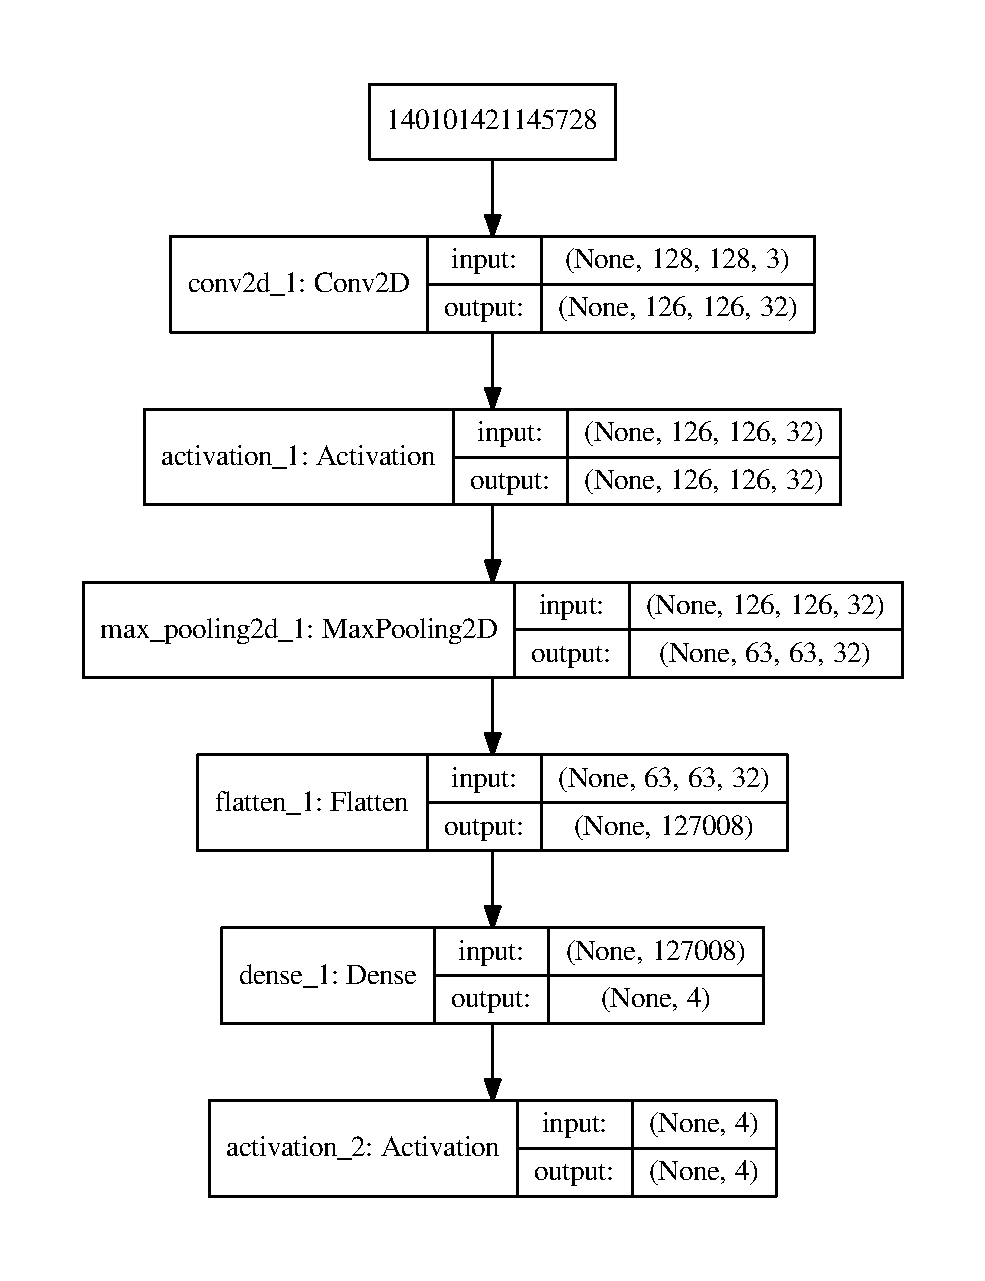
\includegraphics[scale=0.5]{model0_plot.pdf}
\caption{The architecture of model 0.}
\label{fig: model0}
\end{figure}

\newpage
\begin{figure}[h]
\centering
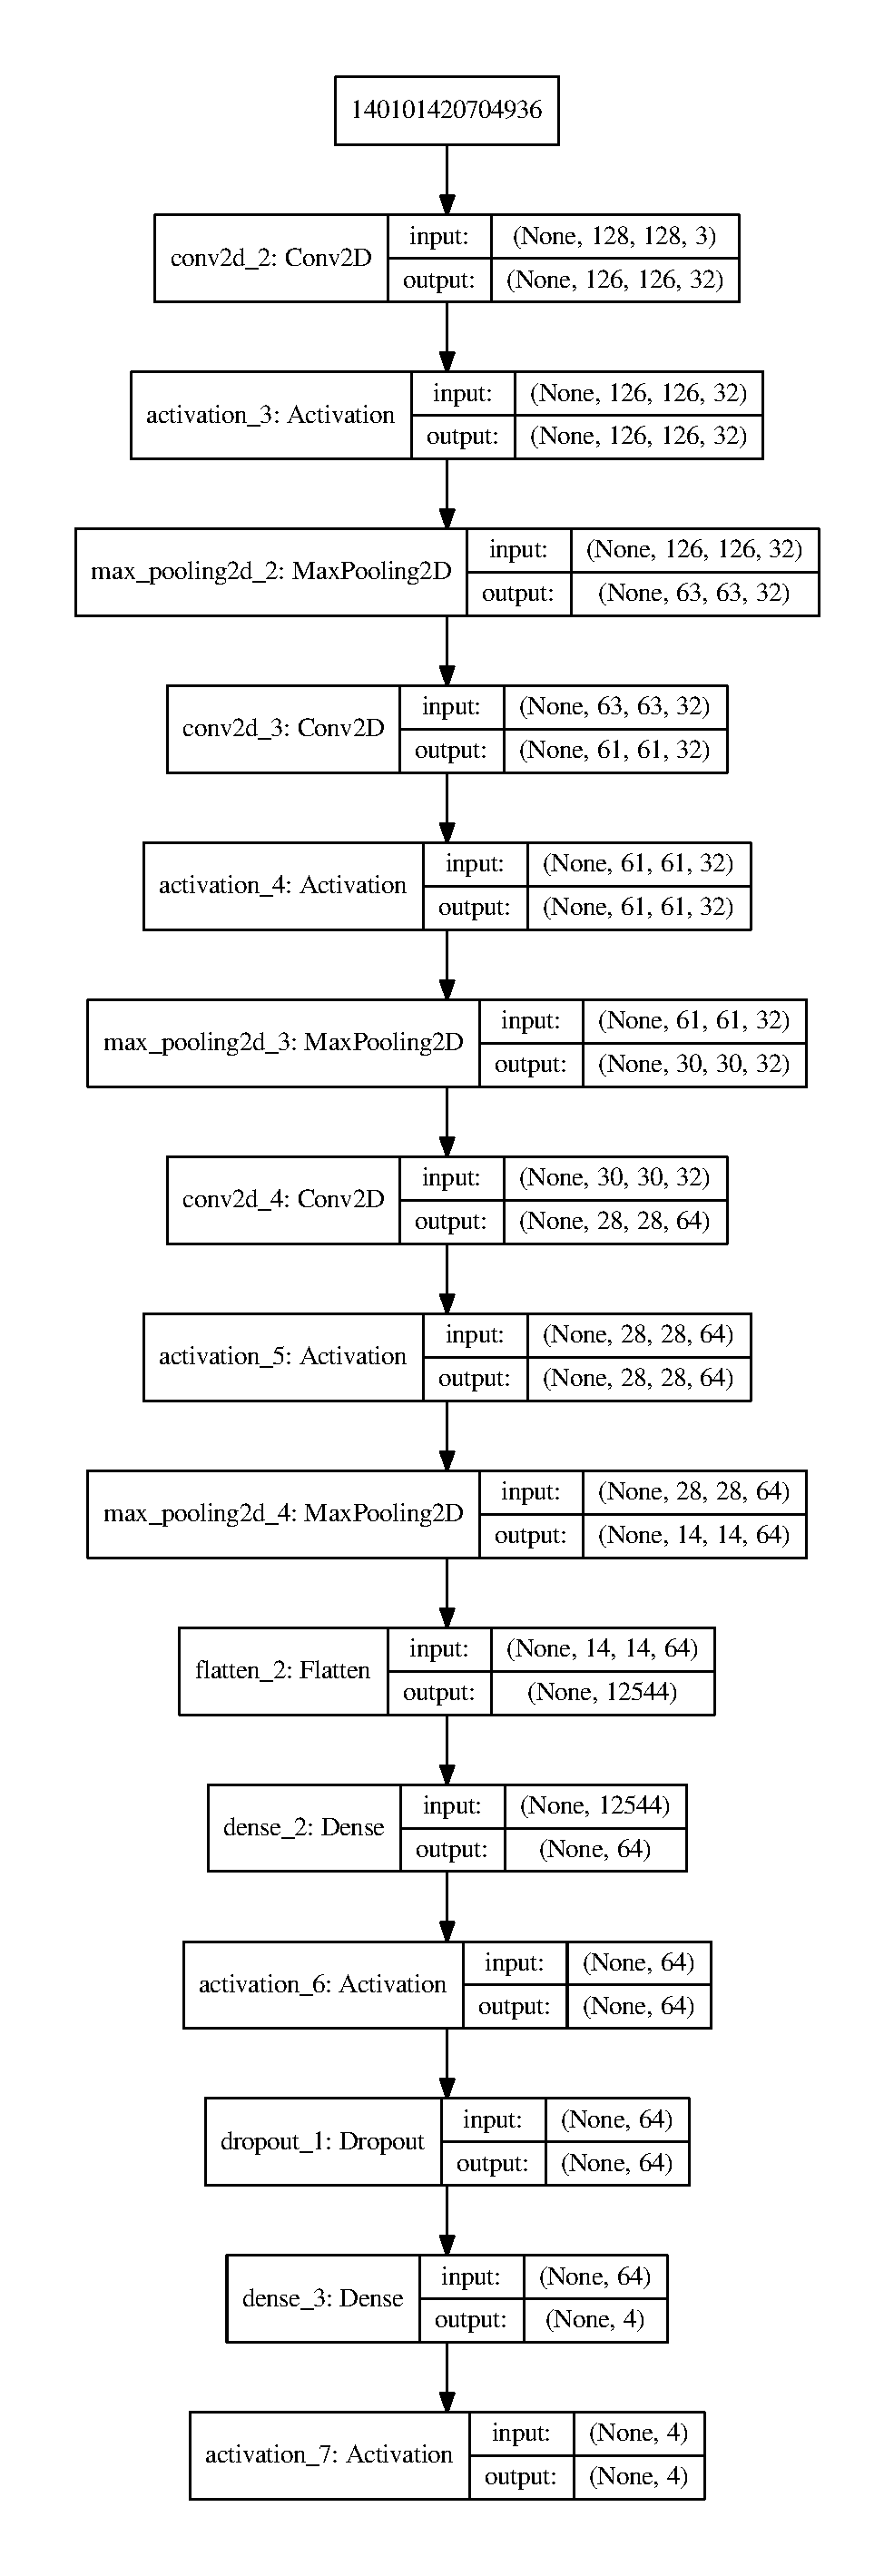
\includegraphics[scale=0.43]{model1_plot.pdf}
\caption{The architecture of model 1.}
\label{fig: model1}
\end{figure}

\newpage
\begin{figure}[h]
\centering
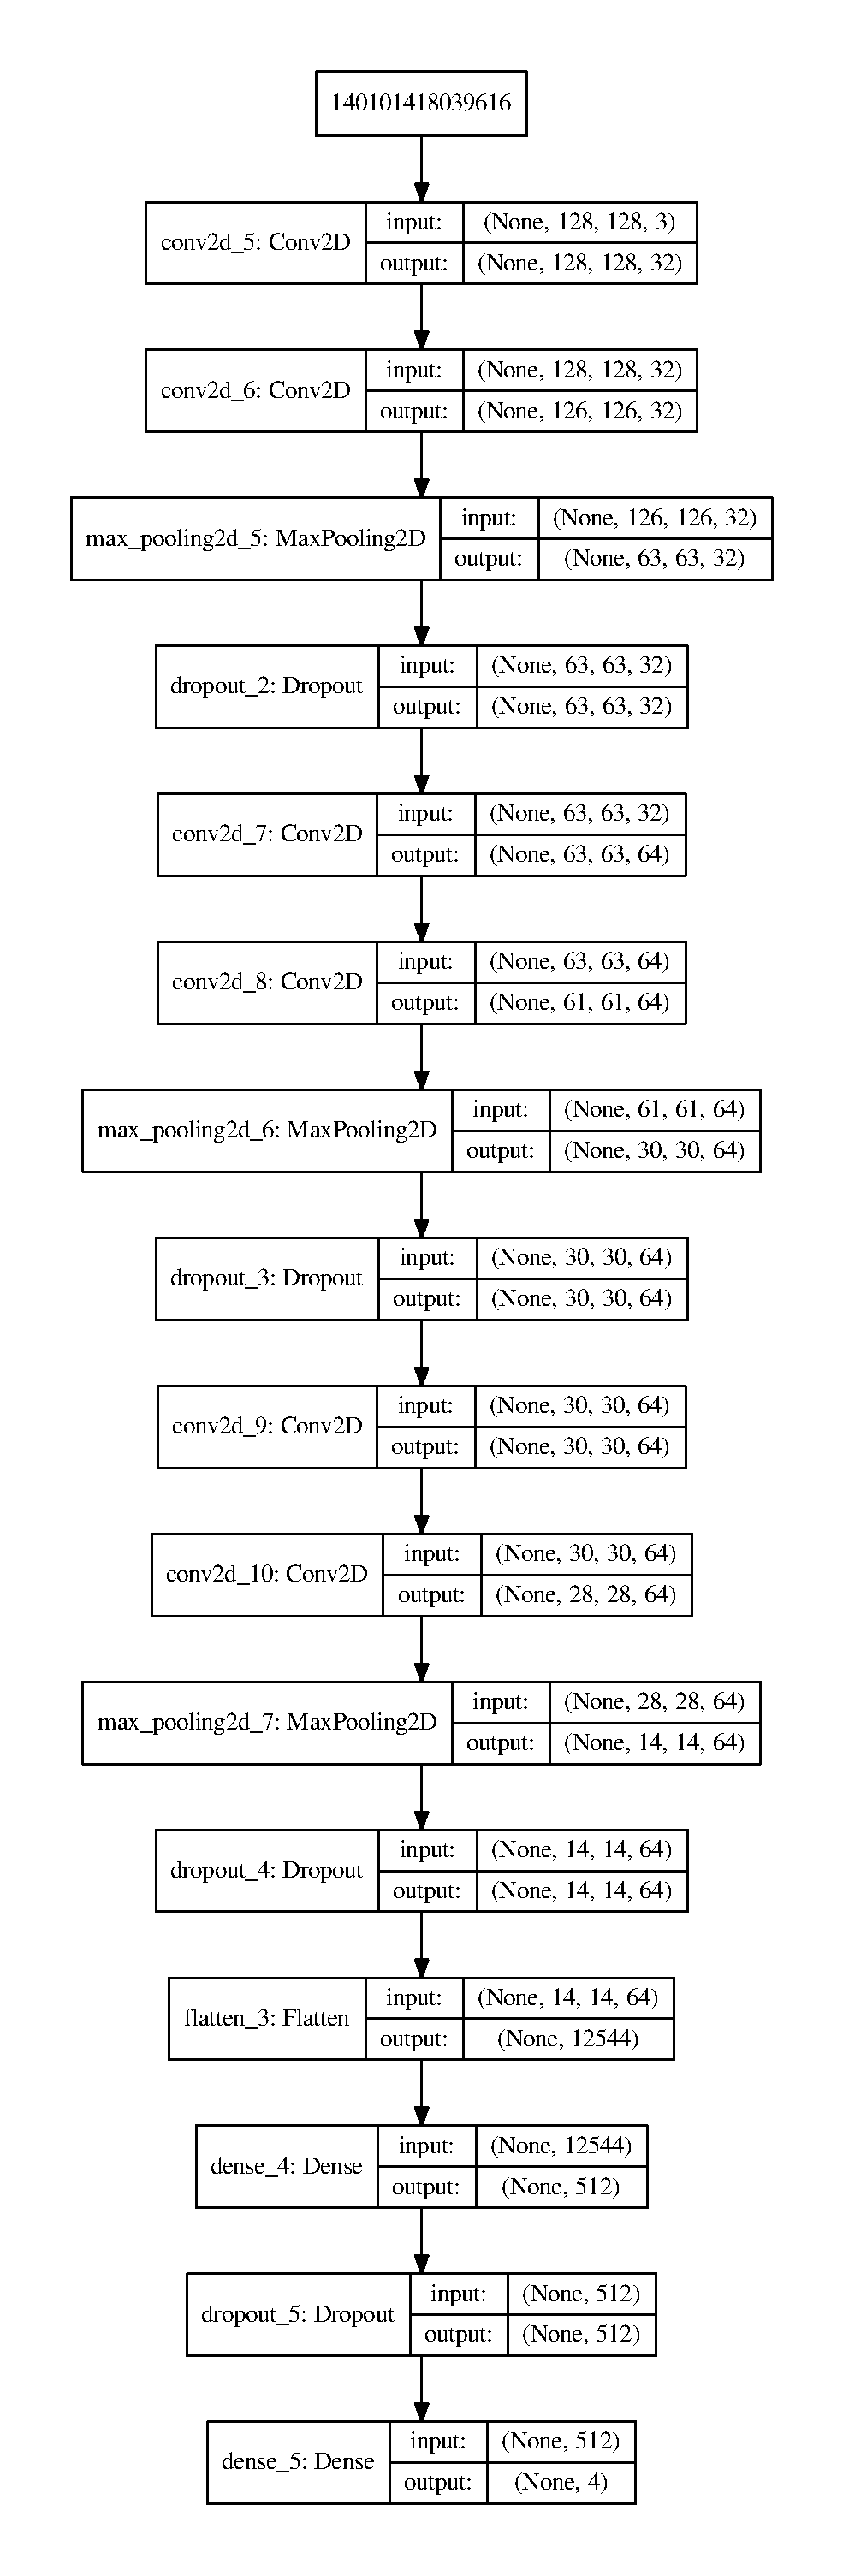
\includegraphics[scale=0.43]{model2_plot.pdf}
\caption{The architecture of model 2.}
\label{fig: model2}
\end{figure}


\end{document}